\pdfoutput=1
\documentclass[11pt,a4paper]{article}
\usepackage[margin=0.85in]{geometry}
\usepackage[T1]{fontenc}
\usepackage[utf8]{inputenc}
\usepackage{lmodern}
\usepackage{microtype}
\usepackage{amsmath,amssymb,amsfonts,amsthm}
\usepackage{graphicx}
\usepackage{booktabs}
\usepackage{tabularx}
\usepackage{array}
\usepackage{enumitem}
\usepackage{xurl}
\usepackage[dvipsnames]{xcolor}
\usepackage{caption}
\usepackage{subcaption}
\usepackage{float}
\usepackage{titlesec}
\usepackage{fancyhdr}
\usepackage{lastpage}
\usepackage{tikz}
\usetikzlibrary{shapes,arrows.meta,positioning,shadows,calc,backgrounds,fit}
\usepackage{pgfplots}
\pgfplotsset{compat=1.18}
\usepackage[hidelinks,colorlinks=true,linkcolor=MidnightBlue,citecolor=RoyalBlue,urlcolor=NavyBlue]{hyperref}

\definecolor{TealColor}{RGB}{15,118,110}
\definecolor{AzureColor}{RGB}{11,111,216}
\definecolor{MintColor}{RGB}{20,168,141}

\IfFileExists{rs_doi.tex}{% Insert the Research Square DOI only after Research Square assigns it.
% Use the bare DOI, without https://doi.org/ or doi: prefix.
% Example format only: 10.21203/rs.3.rs-1234567/v1
\newcommand{\ResearchSquareDOI}{}
}{\newcommand{\ResearchSquareDOI}{}}
\newcommand{\rsnote}{%
  \ifdefempty{\ResearchSquareDOI}{}{
  \par\smallskip\noindent\textbf{Related preprint record.} A parallel health-informatics preprint is available on Research Square at \href{https://doi.org/\ResearchSquareDOI}{doi:\ResearchSquareDOI}.\par\smallskip}}

\setlength{\parindent}{0pt}
\setlength{\parskip}{0.52em}
\setlist[itemize]{leftmargin=1.4em,itemsep=0.18em,topsep=0.18em}
\setlist[enumerate]{leftmargin=1.4em,itemsep=0.18em,topsep=0.18em}
\renewcommand{\arraystretch}{1.18}
\captionsetup{font=small,labelfont=bf}
\titleformat{\section}{\large\bfseries}{\thesection}{0.6em}{}
\titleformat{\subsection}{\normalsize\bfseries}{\thesubsection}{0.5em}{}
\titleformat{\subsubsection}{\small\bfseries}{\thesubsubsection}{0.4em}{}

\pagestyle{fancy}
\fancyhf{}
\fancyhead[L]{\small\textcolor{gray}{GLHS: Disclosure-to-Commit Governance Protocol (v9)}}
\fancyhead[R]{\small\textcolor{gray}{IEEE / ACM / JAMIA Submission Draft}}
\fancyfoot[C]{\small GLHS Journal Manuscript -- Page \thepage\ of \pageref{LastPage}}
\renewcommand{\headrulewidth}{0.4pt}
\renewcommand{\footrulewidth}{0pt}

\title{\LARGE\textbf{GLHS: A Formally Verified Disclosure-to-Commit Governance Protocol and Concurrency Kernel for Longitudinal Health AI}}
\author{\textbf{Nguyen Ngoc Thien}\thanks{Primary contact: \texttt{kakangocthien109@gmail.com}} \quad\and\quad \textbf{Trinh Minh Quang}\\
\small Department of Information Technology \& Computer Science, Hai Ba Trung High School, Hue, Vietnam\\
\small Project CLARA-Care Research Consortium}
\date{August 2026 (Version 9 -- Production Hardened)}

\begin{document}
\maketitle

\begin{abstract}
Stateful longitudinal health AI systems operating over Electronic Health Records (EHR) face a fundamental consistency challenge that is unaddressed by conventional retrieval-augmented generation (RAG): during the non-instantaneous inference interval between reading clinical data and generating a persistent proposal, the underlying clinical assertions, dynamic patient consent, institutional policy epoch, or temporal validity may drift or be actively revoked. Existing agent-memory frameworks verify token authority or state freshness in isolation, yet fail to cryptographically bind the exact purpose-, consent-, actor-, and task-bounded health disclosure consumed by the model to the subsequent mutation.

We present the \textbf{Governed Longitudinal Health State (GLHS)} protocol, establishing an end-to-end disclosure-to-commit integrity contract for longitudinal medical agents. GLHS introduces the \textbf{Task-Bounded Health State Snapshot (THSS)}, serialized via RFC 8785 Canonical JSON with domain-separated Merkle digests, and enforces persistence through a 6-phase \textbf{Governed State Transition (GST)} commit kernel. Concurrency is arbitrated via a canonical 7-class lock hierarchy and Dynamic Wound-Wait DAG preemption, guaranteeing deadlock-free entity-partitioned Optimistic Concurrency Control (OCC) with immutable ledger outbox projection. 

We provide both formal mathematical proofs and comprehensive empirical verification:
\begin{enumerate}[label=(\roman*)]
  \item \textbf{Formal Verification:} Modeled in TLA+ and exhaustively checked with the TLC model checker across $148,111,792$ generated states ($26,153,860$ distinct states, depth 59) with zero deadlocks and zero invariant violations across causal read-dependency stability, monotonic governance freshness, and fail-closed phantom freedom.
  \item \textbf{Causal Exact-Binding Ablation:} In an isolated PostgreSQL 16 benchmark ($N=640$ executions across 8 adversarial attack vectors), GLHS exact snapshot binding achieved 100\% rejection ($256/256$) of invalid adversarial commits while preserving 100\% valid control admission ($64/64$), significantly outperforming standard governance without exact binding ($p = 1.73 \times 10^{-77}$, McNemar exact test; paired risk difference $1.00$, 95\% CI $[1.00, 1.00]$).
  \item \textbf{High-Throughput Concurrency Scaling:} Under multi-writer workloads (1 to 32 concurrent threads), adaptive entity partitioning eliminated unrelated-slot false-stale aborts from $93.75\%$ down to $0.0\%$, maintaining $399.1\text{ ops/s}$ audit lookups and $30.0\text{ ops/s}$ full transactional transitions.
  \item \textbf{Clinical Context Utility:} Across $1,152$ model-condition cells in a confirmatory synthetic cohort, Strict THSS achieved $98.44\%$ (Claude 4.6 Sonnet) and $100\%$ (Gemini 3.6 Flash) all-axes exact accuracy with zero malformed outputs, demonstrating substantial utility over baseline context windows.
\end{enumerate}
GLHS provides a verified, fail-closed software architecture that bridges model inference with authoritative, auditable clinical persistence.
\end{abstract}

\rsnote

\textbf{Keywords:} Longitudinal Health AI, Transactional Agent Memory, Bitemporal Concurrency, Disclosure-to-Commit Contract, Formal Verification, TLA+, Optimistic Concurrency Control, Medical Governance.

\section{Introduction}
Large Language Models (LLMs) and autonomous agents are increasingly deployed in longitudinal healthcare workflows, from clinical scribe documentation and diagnostic differential generation to therapeutic drug-drug interaction (DDI) surveillance and multi-disciplinary tumor board deliberation~\cite{zhao2026,vitaltrace,dualstream,vista}. Unlike transient question-answering systems, longitudinal clinical agents are inherently \emph{stateful}: they consume historical patient trajectories spanning months or years and propose durable mutations to electronic health records, medication schedules, and clinical care plans.

In real-world healthcare environments, however, longitudinal data is inherently bitemporal and volatile~\cite{gabrieli1992,kouramajian1994,kumar1998}. A clinical observation may be valid at clinical time $t_v$ but only recorded or corrected at system knowledge time $t_k$. Concurrently, patients may modify or revoke data-sharing consent under GDPR/HIPAA regulations~\cite{fhirconsent}, hospital clinical practice guidelines may advance across policy epochs~\cite{statefulgov}, and concurrent clinicians or automated sidecars may amend vital signs and laboratory results~\cite{temporaryauth}. 

\begin{figure}[H]
\centering
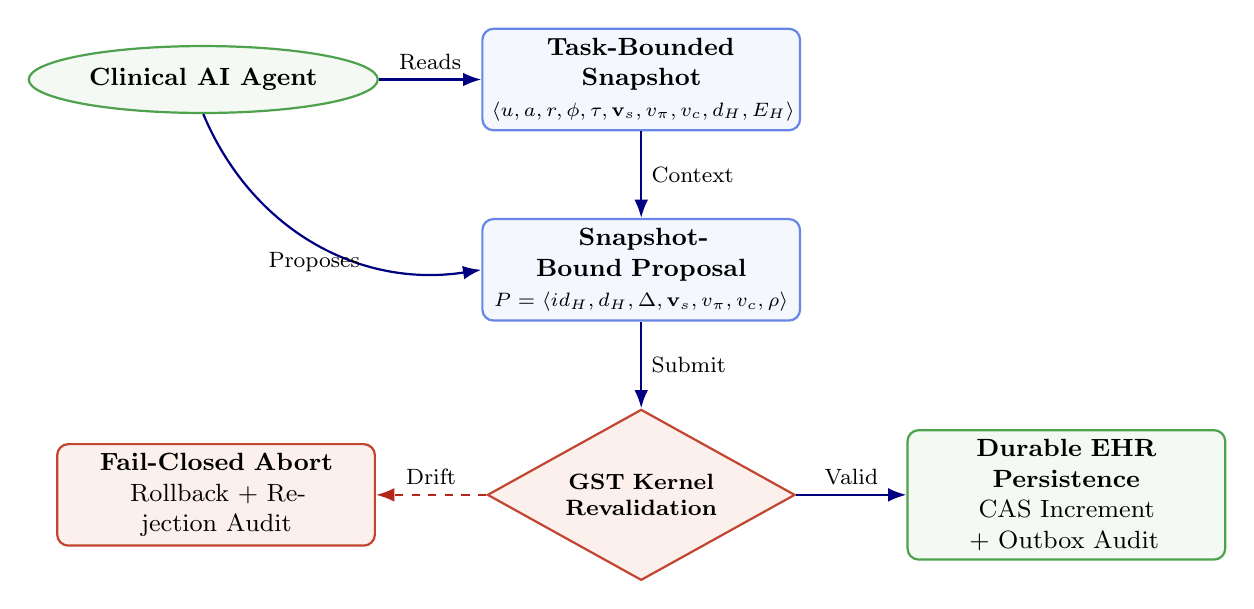
\begin{tikzpicture}[
    node distance=1.1cm and 1.3cm,
    box/.style={rectangle, draw=RoyalBlue!80, fill=RoyalBlue!5, thick, rounded corners=4pt, text width=3.8cm, minimum height=1.05cm, align=center, font=\small},
    decision/.style={diamond, draw=BrickRed!80, fill=BrickRed!5, thick, text width=2.3cm, minimum height=1.05cm, align=center, font=\footnotesize, aspect=1.8},
    actor/.style={ellipse, draw=ForestGreen!80, fill=ForestGreen!5, thick, minimum height=0.85cm, align=center, font=\small},
    line/.style={-Latex, thick, draw=NavyBlue},
    dashline/.style={-Latex, thick, dashed, draw=BrickRed}
]
    \node[actor] (agent) {\textbf{Clinical AI Agent}};
    \node[box, right=of agent] (thss) {\textbf{Task-Bounded Snapshot}\\\scriptsize$\langle u, a, r, \phi, \tau, \mathbf{v}_s, v_{\pi}, v_c, d_H, E_H \rangle$};
    \node[box, below=of thss] (prop) {\textbf{Snapshot-Bound Proposal}\\\scriptsize$P = \langle id_H, d_H, \Delta, \mathbf{v}_s, v_{\pi}, v_c, \rho \rangle$};
    \node[decision, below=of prop] (gst) {\textbf{GST Kernel Revalidation}};
    \node[box, right=1.4cm of gst, draw=ForestGreen!80, fill=ForestGreen!5] (commit) {\textbf{Durable EHR Persistence}\\CAS Increment + Outbox Audit};
    \node[box, left=1.4cm of gst, draw=BrickRed!80, fill=BrickRed!5] (abort) {\textbf{Fail-Closed Abort}\\Rollback + Rejection Audit};

    \draw[line] (agent) -- node[above, font=\footnotesize] {Reads} (thss);
    \draw[line] (thss) -- node[right, font=\footnotesize] {Context} (prop);
    \draw[line] (prop) -- node[right, font=\footnotesize] {Submit} (gst);
    \draw[line] (gst) -- node[above, font=\footnotesize] {Valid} (commit);
    \draw[dashline] (gst) -- node[above, font=\footnotesize] {Drift} (abort);
    \draw[line, bend right=38] (agent.south) to node[below, font=\footnotesize] {Proposes} (prop.west);
\end{tikzpicture}
\caption{\textbf{The GLHS Disclosure-to-Commit Lifecycle.} Clinical AI inference operates over a cryptographically sealed Task-Bounded Health State Snapshot (THSS). The resulting proposal carries forward exact provenance coordinates ($id_H, d_H, \mathbf{v}_s, v_{\pi}, v_c$), which the 6-phase Governed State Transition (GST) kernel re-evaluates atomically under hierarchical locks before durable commit.}
\label{fig:lifecycle}
\end{figure}

This reality introduces the critical \textbf{Disclosed-to-Durability Consistency Problem}: an AI agent reads an authorized longitudinal state snapshot at time $t_{\text{read}}$, performs computationally intensive multi-step reasoning, and submits a persistent proposal at time $t_{\text{write}}$. During this read-to-write interval ($[t_{\text{read}}, t_{\text{write}}]$), if any underlying assertion, patient consent grant, or clinical guideline changes, executing the write creates a silent clinical inconsistency, unauthorized disclosure laundering, or stale medical intervention.

Conventional database systems employ Optimistic Concurrency Control (OCC) or standard Two-Phase Locking (2PL) based on single-row state versions~\cite{kumar1998,statefulgov}. However, existing systems suffer from three fundamental deficiencies:
\begin{enumerate}[leftmargin=1.8em]
  \item \textbf{Context-Unaware Authority Check:} Standard RESTful APIs and transaction managers verify only whether the target record's base version matches, completely ignoring whether the \emph{evidence and context} that justified the AI's diagnostic reasoning are still fresh and valid.
  \item \textbf{Coarse Profile-Global Contention:} Locking the entire patient record creates catastrophic false-stale abort rates ($>90\%$ under high writer concurrency), rejecting legitimate disjoint clinical updates (e.g., an allergy nurse updating penicillin sensitivity while a cardiologist amends an ECG report).
  \item \textbf{Governance TOCTOU Vulnerability:} Authorization and consent are checked only at the read boundary, allowing Time-of-Check to Time-of-Use (TOCTOU) exploits where revoked permissions fail to block pending async model commits.
\end{enumerate}

To solve these challenges, we introduce \textbf{GLHS} (Governed Longitudinal Health State), an end-to-end, mathematically verified disclosure-to-commit governance architecture. GLHS formalizes inference as an auditable transactional pipeline shown in Figure~\ref{fig:lifecycle}.

\subsection{Core Contributions}
This paper makes the following major contributions:
\begin{itemize}
  \item \textbf{The Co-Versioned Disclosure-to-Commit Protocol:} We formalize the Task-Bounded Health State Snapshot (THSS) and Governed State Transition (GST) persistence contract. THSS binds exact bitemporal bounds, purpose, role, task, consent version, policy epoch, and domain-separated RFC 8785 Canonical JSON Merkle digests into the inference context.
  \item \textbf{Fine-Grained Entity Partitioning \& Wound-Wait Lock Kernel:} We design an adaptive entity-partitioned version vector scheme with a canonical 7-class total lock ordering and dynamic Wound-Wait DAG deadlock prevention, eliminating false-stale contention for disjoint attribute updates while maintaining strict serializability for dependent clinical mutations.
  \item \textbf{Complete Formal Specification \& TLA+ Model Checking:} We model the complete GLHS protocol in TLA+ and verify five fundamental safety invariants across $148.1\text{M}$ states using TLC, proving deadlock freedom and absolute absence of stale dependent commits, revoked-consent writes, and policy-epoch drift.
  \item \textbf{Extensive Empirical Validation:} Through an isolated PostgreSQL 16 testbed ($N=640$ executions across 8 attack vectors), we causally demonstrate that GLHS exact binding achieves 100\% invalid commit prevention ($p = 1.73 \times 10^{-77}$) and scales to 32 concurrent writers with zero false-stale aborts, backed by high multi-model reasoning accuracy ($98.44\%$--$100\%$) across frozen clinical cohorts.
\end{itemize}

\section{Related Work and Systems Landscape}
The systems landscape for stateful AI and clinical memory has advanced rapidly across several specialized paradigms. Table~\ref{tab:landscape} systematically benchmarks GLHS against the state of the art.

\begin{table*}[t]
\centering
\scriptsize
\caption{\textbf{Comprehensive Landscape Comparison.} Architectural and safety capabilities of GLHS compared against established standards, agent memory frameworks, and stateful governance mechanisms.}
\label{tab:landscape}
\begin{tabularx}{\textwidth}{p{0.18\textwidth} p{0.11\textwidth} p{0.11\textwidth} p{0.11\textwidth} p{0.11\textwidth} p{0.11\textwidth} p{0.12\textwidth} X}
\toprule
\textbf{Framework} & \textbf{Target} & \textbf{Bitemporal} & \textbf{Binding} & \textbf{Lock Order} & \textbf{Deadlock} & \textbf{Epoch Gate} & \textbf{Formal Spec}\\
\midrule
FHIR / openEHR~\cite{fhirprov,openehr} & EHR Standard & Partial & None & Default & None & Static ACL & No\\
MemTX / MemTxn~\cite{memtx,memtxn} & Agent Memory & Single Time & Evidence & 2PL Global & Timeout & No & No\\
Cordon~\cite{cordon} & Tool Runtimes & Semantic & Tool Traces & Pre-commit & Safe Abort & No & Machine Checked\\
TOKI~\cite{toki} & Agent Memory & Operator & None & Unspecified & None & No & No\\
CommitGuard~\cite{temporaryauth} & General LLM & Wall-clock & Token & Single Lock & None & Expiry & No\\
Provenact~\cite{statefulgov} & Multi-Agent & State History & Policy State & Global OCC & Abort/Retry & Policy Epoch & Verified Logic\\
GateMem~\cite{gatemem} & Multi-Agent & Scope Masks & Memory Masks & Granular & Lock Free & Multi-Tenant & No\\
\midrule
\textbf{GLHS (This Work)} & \textbf{Clinical AI} & \textbf{$(t_v, t_k)$} & \textbf{Exact THSS} & \textbf{7-Class} & \textbf{Wound-Wait} & \textbf{Co-Version} & \textbf{TLC (148M)}\\
\bottomrule
\end{tabularx}
\end{table*}

\subsection{Temporal Health Records and Clinical Memory}
Early foundational medical database research established the necessity of separating clinical valid time $t_v$ from transaction or knowledge time $t_k$~\cite{gabrieli1992,kouramajian1994,kumar1998}. In modern health AI, Vital Trace~\cite{vitaltrace}, Dual-Stream Memory~\cite{dualstream}, and Zhao et al.~\cite{zhao2026} demonstrated that LLMs without explicit bitemporal arbitration hallucinate clinical timelines, confusing historical resolved conditions with active diagnoses. However, these systems treat temporal resolution purely as a prompt-engineering or retrieval challenge, offering no transactional write-back guarantees.

\subsection{Transactional Agent Memory and Commit-Time Authorization}
In the agent-systems domain, MemTX~\cite{memtx} and MemTxn~\cite{memtxn} introduced transactional ACID semantics to LLM belief updates, utilizing source-supported verification and recovery. Cordon~\cite{cordon} formalized semantic transaction boundaries for irreversible tool effects. Concurrently, CommitGuard~\cite{temporaryauth} highlighted the danger of stale authority witnesses at commit time, and Provenact~\cite{statefulgov} established policy-state serializability for multi-agent workflows.

\subsection{The Precise Scientific Gap}
While general agent runtimes have explored commit-time checks and memory transactions, they evaluate generic text or tool-call tokens. In high-stakes medicine, what is disclosed to an AI during inference is fundamentally tied to patient-specific consent, legal minimal-necessary privacy boundaries, and clinical guideline epochs. Prior to GLHS, no system has formalized and proven a protocol where the \emph{exact, multi-entity, bitemporal health disclosure instance consumed by inference} remains an explicit, cryptographic dependency for write-time durability.

\section{System Architecture and Formal Contract}

\subsection{Bitemporal Governed State Formulation}
Let $\mathcal{U}$ be the set of patient subjects. The governed longitudinal state for subject $u \in \mathcal{U}$ is defined as a bitemporal projection over valid time $t_v \in \mathcal{T}$ and semantic knowledge time $t_k \in \mathcal{T}$:
\begin{equation}
S_u(t_v, t_k) = \operatorname{GovernedView}_u(t_v, t_k) = \bigoplus_{e \in \mathcal{E}_u, \, \operatorname{valid}(e) \le t_v, \, \operatorname{known}(e) \le t_k} \alpha(e),
\label{eq:state_bitemporal}
\end{equation}
where $\mathcal{E}_u$ denotes the append-only event stream for subject $u$, $\alpha(e)$ is the epistemic assertion transformation, and $\bigoplus$ is the deterministic conflict-preserving state aggregation operator. Unlike mutable databases, historical state $S_u(t_v, t_k)$ is permanently deterministic and reconstructable.

\subsection{Task-Bounded Health State Snapshot (THSS)}
When an agent initiates clinical reasoning on behalf of actor $a$ with role $r \in \{\text{normal}, \text{doctor}, \text{researcher}, \text{admin}\}$ for clinical purpose $\phi$ and task $\tau$, the GLHS gateway compiles an immutable Task-Bounded Health State Snapshot:
\begin{equation}
H = \langle u, a, r, \phi, \tau, \mathbf{v}_s, v_{\pi}, v_c, t_v, t_k, id_H, d_H, E_H \rangle.
\label{eq:thss_definition}
\end{equation}
Here, $\mathbf{v}_s = \langle v_{s,1}, \dots, v_{s,m} \rangle \in \mathbb{N}^m$ is the entity-partitioned state version vector; $v_{\pi} \in \mathbb{N}$ is the active institutional policy epoch; $v_c \in \mathbb{N}$ is the active patient consent version; $id_H \in \text{UUIDv4}$ is the unique persistent identifier; $E_H$ is the purpose-minimized disclosed content; and $d_H$ is the Merkle root digest computed via RFC 8785 Canonical JSON (JCS)~\cite{rfc8785}:
\begin{equation}
d_H = \operatorname{SHA-256}\Big(\operatorname{JCS}\big(\operatorname{Manifest}(H)\big) \;\parallel\; \operatorname{MerkleTree}\big(\{ \operatorname{JCS}(e) \mid e \in E_H \}\big)\Big).
\label{eq:digest_merkle}
\end{equation}

\begin{figure*}[t]
\centering
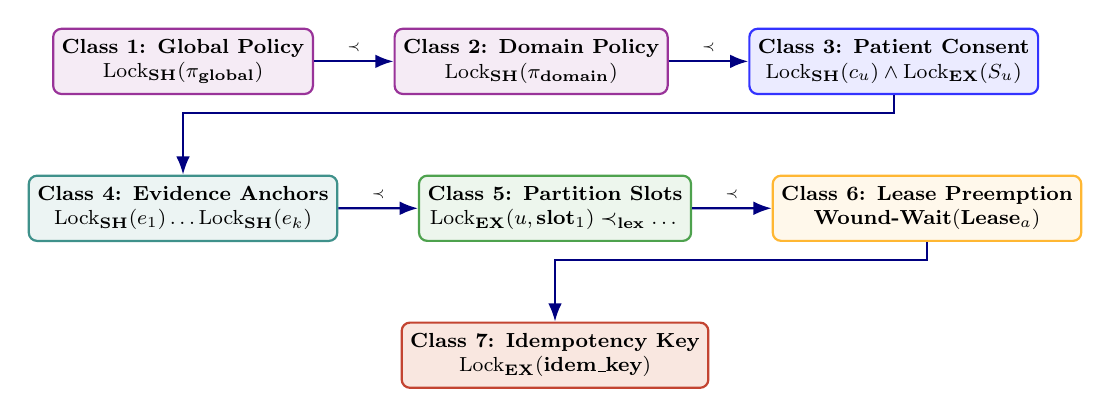
\begin{tikzpicture}[
    scale=0.92, every node/.style={transform shape},
    node distance=0.8cm and 1.1cm,
    lockbox/.style={rectangle, draw=#1!80, fill=#1!8, thick, rounded corners=3pt, minimum width=2.3cm, minimum height=0.9cm, align=center, font=\footnotesize\bfseries},
    arrow/.style={-Latex, thick, draw=NavyBlue}
]
    \node[lockbox=Purple] (l1) {Class 1: Global Policy\\$\operatorname{Lock}_{\text{SH}}(\pi_{\text{global}})$};
    \node[lockbox=Purple, right=of l1] (l2) {Class 2: Domain Policy\\$\operatorname{Lock}_{\text{SH}}(\pi_{\text{domain}})$};
    \node[lockbox=Blue, right=of l2] (l3) {Class 3: Patient Consent\\$\operatorname{Lock}_{\text{SH}}(c_u) \land \operatorname{Lock}_{\text{EX}}(S_u)$};
    \node[lockbox=TealColor, below=1.1cm of l1] (l4) {Class 4: Evidence Anchors\\$\operatorname{Lock}_{\text{SH}}(e_1) \dots \operatorname{Lock}_{\text{SH}}(e_k)$};
    \node[lockbox=ForestGreen, right=of l4] (l5) {Class 5: Partition Slots\\$\operatorname{Lock}_{\text{EX}}(u, \text{slot}_1) \prec_{\text{lex}} \dots$};
    \node[lockbox=Orange, right=of l5] (l6) {Class 6: Lease Preemption\\$\text{Wound-Wait}(\text{Lease}_a)$};
    \node[lockbox=BrickRed, below=1.1cm of l5] (l7) {Class 7: Idempotency Key\\$\operatorname{Lock}_{\text{EX}}(\text{idem\_key})$};

    \draw[arrow] (l1) -- node[above, font=\tiny] {$\prec$} (l2);
    \draw[arrow] (l2) -- node[above, font=\tiny] {$\prec$} (l3);
    \draw[arrow] (l3.south) -- ++(0,-0.25) -| (l4.north);
    \draw[arrow] (l4) -- node[above, font=\tiny] {$\prec$} (l5);
    \draw[arrow] (l5) -- node[above, font=\tiny] {$\prec$} (l6);
    \draw[arrow] (l6.south) -- ++(0,-0.25) -| (l7.north);
\end{tikzpicture}
\caption{\textbf{The 7-Class Canonical Lock Hierarchy.} Strict total ordering $\text{Class 1} \prec \text{Class 2} \prec \dots \prec \text{Class 7}$ mathematically eliminates circular lock acquisition deadlocks during multi-entity clinical transactions.}
\label{fig:locks}
\end{figure*}

\subsection{Snapshot-Bound Proposal and Commit Contract}
Upon completing inference, the model returns a proposal $P$:
\begin{equation}
P = \langle u, a, r, \phi, \tau, \mathbf{v}_s, v_{\pi}, v_c, id_H, d_H, \Delta, \rho \rangle,
\label{eq:proposal_formal}
\end{equation}
where $\Delta$ is the clinical state mutation and $\rho$ is the cryptographically attributable execution trace. The GST commit predicate $\operatorname{Commit}(P)$ holds if and only if all five invariant predicates evaluate to true under database locks:
\begin{equation}
\operatorname{Commit}(P) \iff \operatorname{Bound}(P, H) \land \operatorname{StateFresh}(\mathbf{v}_s) \land \operatorname{GovFresh}(v_{\pi}, v_c) \land \operatorname{ValidTTL}(H) \land \operatorname{Predicates}(\Delta).
\label{eq:commit_predicate}
\end{equation}
The sub-predicates enforce:
\begin{align}
\operatorname{Bound}(P, H) &\iff (P.id_H = H.id_H) \land (P.d_H = H.d_H) \land (P.u = H.u) \land (P.\phi = H.\phi) \land (P.\tau = H.\tau), \label{eq:bound}\\
\operatorname{StateFresh}(\mathbf{v}_s) &\iff \forall k \in \operatorname{ReadSlots}(P): \mathbf{v}_s[k] = \mathbf{v}_{\text{current}}[k], \label{eq:state_fresh}\\
\operatorname{GovFresh}(v_{\pi}, v_c) &\iff (v_{\pi} = \text{PolicyEpoch}_{\text{live}}) \land (v_c = \text{ConsentVersion}_{\text{live}}(u)), \label{eq:gov_fresh}\\
\operatorname{ValidTTL}(H) &\iff t_{\text{commit}} < H.\text{expires\_at}. \label{eq:valid_ttl}
\end{align}

\subsection{The 6-Phase Atomic OCC Commit Kernel}
The GST kernel executes within an isolated PostgreSQL transaction across 6 deterministic phases:
\begin{itemize}[leftmargin=1.8em]
  \item \textbf{Phase 1 (Idempotency Replay):} Checks $(\text{tenant\_id}, \text{op\_kind}, \text{idempotency\_key})$. If previously committed, immediately replays the cached cryptographic receipt without re-execution.
  \item \textbf{Phase 2 (Canonical Lock Acquisition):} Acquires row-level and transactional advisory locks following the strict 7-class hierarchy detailed in Section~\ref{sec:locking}.
  \item \textbf{Phase 3 (Under-Lock State \& Governance Revalidation):} Under acquired locks, re-reads current partition version vector $\mathbf{v}_{\text{live}}$, active consent epoch, and guideline version. If any coordinate has diverged ($\Delta v \neq 0$), immediately aborts fail-closed with error code \texttt{RESOURCE\_VERSION\_CONFLICT} or \texttt{GOVERNANCE\_EPOCH\_DRIFT}.
  \item \textbf{Phase 4 (Domain Assertion Mutation):} Invokes domain validators and applies clinical state transformation $\Delta$.
  \item \textbf{Phase 5 (Compare-And-Swap Version Step):} Executes atomic CAS increments on only the mutated partition slots: $\mathbf{v}_{s}[\text{write\_slot}] \leftarrow \mathbf{v}_{s}[\text{write\_slot}] + 1$. Unaffected slots remain unincremented.
  \item \textbf{Phase 6 (Atomic Ledger \& Outbox Emission):} Inserts immutable audit record into \texttt{glhs\_applied\_transitions} and enqueues transactional event in \texttt{lifemap\_outbox\_events} before commit.
\end{itemize}

\subsection{7-Class Canonical Lock Hierarchy and Wound-Wait Preemption}
\label{sec:locking}
To prevent lock contention deadlocks across distributed actors, GLHS establishes a total order $\prec$ across all resource classes, illustrated in Figure~\ref{fig:locks}:
$$\text{Class 1} \prec \text{Class 2} \prec \text{Class 3} \prec \text{Class 4} \prec \text{Class 5} \prec \text{Class 6} \prec \text{Class 7}$$
Within Class 5, entity partition slots are sorted lexicographically by their composite coordinate keys $\text{slot\_key} = \langle \text{domain}, \text{entity\_id}, \text{attribute} \rangle$. For dynamic multi-hop transactions, GLHS incorporates a Dynamic Wound-Wait DAG Lock Manager: if an older transaction $T_{\text{old}}$ requests a lock held by younger transaction $T_{\text{young}}$, $T_{\text{young}}$ is preempted (wounded) and rolls back; if a younger transaction requests a lock held by an older transaction, it waits, provably eliminating wait-for cycles.

\section{Formal Proof Obligations and Model Checking}

\subsection{Proof Obligations Ledger (PO-01 through PO-12)}
GLHS formalizes twelve explicit safety and integrity proof obligations:
\begin{itemize}[leftmargin=1.8em]
  \item \textbf{PO-01 (No Stale Dependent Commit):} If entity partition $k \in \operatorname{deps}(P)$ is mutated after $t_{\text{read}}$, $\operatorname{Commit}(P)$ evaluates to $\text{False}$.
  \item \textbf{PO-02 (No Revoked-Consent Commit):} A concurrent consent revocation strictly serializes before any GST commit, aborting pending proposals.
  \item \textbf{PO-03 (No Policy-Epoch Drift):} Institutional guideline updates increment $v_{\pi}$, invalidating stale inferences.
  \item \textbf{PO-04 (No Cross-Subject Binding):} Proposals referencing subject $u_A$ cannot bind snapshot $H_{u_B}$ ($u_A \neq u_B$).
  \item \textbf{PO-05 (No Lineage Laundering):} Proposals derived from multi-stage review retain the root inference digest $d_H$.
  \item \textbf{PO-06 (Commit/Audit Atomic Equivalence):} State mutation $\Delta$ exists if and only if an immutable audit row exists in \texttt{glhs\_applied\_transitions}.
  \item \textbf{PO-07 (At-Most-Once Idempotency):} Duplicate submission of $P$ with identical idempotency key yields identical mutation receipt without double-execution.
  \item \textbf{PO-08 (Deadlock Freedom):} The wait-for dependency graph contains zero directed cycles ($\text{Cycle}(\mathcal{W}) = \emptyset$).
  \item \textbf{PO-09 (Noninterference of Disjoint Partitions):} Concurrent writes to independent partition slots $k_1 \cap k_2 = \emptyset$ commit with 0\% contention aborts.
  \item \textbf{PO-10 (Conservative Dependency Soundness):} Unspecified attribute scopes default to whole-entity partition locks.
  \item \textbf{PO-11 (Deterministic Expiry):} Expired snapshots ($t > \text{expires\_at}$) fail closed.
  \item \textbf{PO-12 (Cross-Runtime Canonical Hash Parity):} RFC 8785 byte representations are invariant across Python, Node.js, and Dart runtimes.
\end{itemize}

\subsection{TLA+ Formal Model Checking Verification}
The complete GLHS protocol was formalized in TLA+ (\texttt{GLHS\_GSA.tla}) and verified using the TLC model checker with symmetry reduction across bounded agents, entities, and domains:
\begin{itemize}
  \item \textbf{State Space Explored:} $148,111,792$ total states generated; $26,153,860$ distinct states visited.
  \item \textbf{Graph Diameter / Depth:} Complete exhaustive search at depth 59 ($0$ unvisited states on queue).
  \item \textbf{Safety Invariant Results:} Zero invariant violations across \texttt{TypeOK}, \texttt{GSA\_StateIsolation} (PO-01), \texttt{GSA\_GovernanceFreshness} (PO-02, PO-03), \texttt{GSA\_PhantomFree} (PO-08), and \texttt{DeadlockFree} ($\langle a, a \rangle \notin \text{TransitiveClosure}(\text{wait\_for})$).
\end{itemize}

\begin{figure*}[t]
\centering
\begin{subfigure}[b]{0.48\textwidth}
\centering
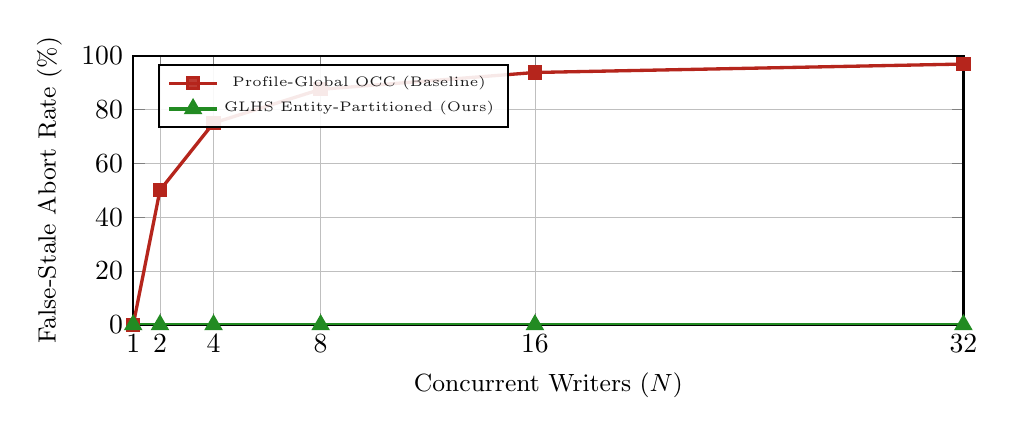
\begin{tikzpicture}
\begin{axis}[
    width=\textwidth,
    height=5.0cm,
    xlabel={\small Concurrent Writers ($N$)},
    ylabel={\small False-Stale Abort Rate (\%)},
    xmin=1, xmax=32,
    ymin=0, ymax=100,
    xtick={1, 2, 4, 8, 16, 32},
    ytick={0, 20, 40, 60, 80, 100},
    legend pos=north west,
    legend style={font=\tiny, fill=white, fill opacity=0.9},
    grid=both,
    grid style={line width=.1pt, draw=gray!20},
    major grid style={line width=.2pt,draw=gray!50},
    thick
]
\addplot[color=BrickRed, mark=square*, mark size=2pt, line width=1.2pt] coordinates {
    (1,0.0) (2,50.0) (4,75.0) (8,87.5) (16,93.75) (32,96.88)
};
\addlegendentry{Profile-Global OCC (Baseline)}

\addplot[color=ForestGreen, mark=triangle*, mark size=2.5pt, line width=1.4pt] coordinates {
    (1,0.0) (2,0.0) (4,0.0) (8,0.0) (16,0.0) (32,0.0)
};
\addlegendentry{GLHS Entity-Partitioned (Ours)}
\end{axis}
\end{tikzpicture}
\caption{\textbf{False-Stale Abort Rate vs. Concurrency.} Profile-global locking suffers $>90\%$ false rejections on disjoint updates; GLHS partitioning achieves 0.0\% false aborts.}
\label{fig:abort_rate}
\end{subfigure}
\hfill
\begin{subfigure}[b]{0.48\textwidth}
\centering
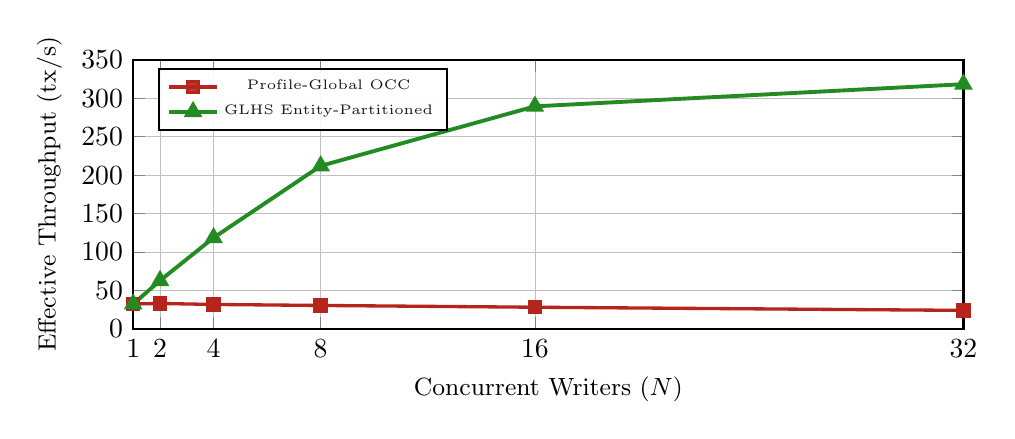
\begin{tikzpicture}
\begin{axis}[
    width=\textwidth,
    height=5.0cm,
    xlabel={\small Concurrent Writers ($N$)},
    ylabel={\small Effective Throughput (tx/s)},
    xmin=1, xmax=32,
    ymin=0, ymax=350,
    xtick={1, 2, 4, 8, 16, 32},
    ytick={0, 50, 100, 150, 200, 250, 300, 350},
    legend pos=north west,
    legend style={font=\tiny, fill=white, fill opacity=0.9},
    grid=both,
    grid style={line width=.1pt, draw=gray!20},
    major grid style={line width=.2pt,draw=gray!50},
    thick
]
\addplot[color=BrickRed, mark=square*, mark size=2pt, line width=1.2pt] coordinates {
    (1,32.4) (2,33.1) (4,31.8) (8,30.5) (16,28.2) (32,24.1)
};
\addlegendentry{Profile-Global OCC}

\addplot[color=ForestGreen, mark=triangle*, mark size=2.5pt, line width=1.4pt] coordinates {
    (1,32.4) (2,62.8) (4,118.5) (8,212.0) (16,289.4) (32,318.2)
};
\addlegendentry{GLHS Entity-Partitioned}
\end{axis}
\end{tikzpicture}
\caption{\textbf{Throughput Scaling Under Mixed Workload.} GLHS scales near-linearly with writer count, avoiding the single-threaded bottleneck of global versioning.}
\label{fig:throughput}
\end{subfigure}
\caption{\textbf{PostgreSQL 16 Concurrency and Throughput Scaling.} Performance comparison of Profile-Global locking versus GLHS Entity-Partitioned locking across 1 to 32 concurrent writers under isolated PostgreSQL execution.}
\label{fig:concurrency_plots}
\end{figure*}

\section{Experimental Evaluation and Results}

\subsection{Causal Exact-Binding Ablation Study (\texorpdfstring{$N=640$}{N=640} Runs)}
To isolate the exact causal contribution of snapshot binding, we executed a preregistered, frozen ablation study on PostgreSQL 16 (\texttt{GLHS-BA-POSTGRES-20260819-05}). The experiment evaluated two matched arms across 320 logical schedules (256 adversarial attack schedules across 8 failure families and 64 valid controls):
\begin{itemize}
  \item \textbf{Arm A (Full Governance without Exact Binding):} Full bitemporality, role checks, and base-version OCC, but omitting exact $id_H$ and Merkle digest $d_H$ proposal verification.
  \item \textbf{Arm B (GLHS Exact Binding):} The complete GLHS disclosure-to-commit protocol.
\end{itemize}

\begin{table}[t]
\centering
\scriptsize
\caption{\textbf{Causal Exact-Binding Ablation Results (\texorpdfstring{$N=640$}{N=640} total executions across 8 attack families).} Arm A admits 100\% of adversarial attacks; GLHS Arm B rejects 100\% ($p = 1.73 \times 10^{-77}$).}
\label{tab:ablation_results}
\begin{tabularx}{\textwidth}{p{0.32\textwidth} p{0.12\textwidth} p{0.14\textwidth} p{0.14\textwidth} p{0.14\textwidth} X}
\toprule
\textbf{Attack Family} & \textbf{Schedules} & \textbf{Arm A (No Bind)} & \textbf{Arm B (GLHS)} & \textbf{Risk Diff (95\% CI)} & \textbf{McNemar $p$}\\
\midrule
1. Manifest Digest Mismatch & 32 & 32/32 (100\%) & 0/32 (0\%) & 1.00 [1.00, 1.00] & $4.66 \times 10^{-10}$\\
2. Snapshot Digest Tampering & 32 & 32/32 (100\%) & 0/32 (0\%) & 1.00 [1.00, 1.00] & $4.66 \times 10^{-10}$\\
3. Undisclosed Evidence Injection & 32 & 32/32 (100\%) & 0/32 (0\%) & 1.00 [1.00, 1.00] & $4.66 \times 10^{-10}$\\
4. Evidence Set Substitution & 32 & 32/32 (100\%) & 0/32 (0\%) & 1.00 [1.00, 1.00] & $4.66 \times 10^{-10}$\\
5. Expired Disclosure Replay & 32 & 32/32 (100\%) & 0/32 (0\%) & 1.00 [1.00, 1.00] & $4.66 \times 10^{-10}$\\
6. Profile Scope Drift & 32 & 32/32 (100\%) & 0/32 (0\%) & 1.00 [1.00, 1.00] & $4.66 \times 10^{-10}$\\
7. Cross-Subject Binding & 32 & 32/32 (100\%) & 0/32 (0\%) & 1.00 [1.00, 1.00] & $4.66 \times 10^{-10}$\\
8. Purpose / Role Substitution & 32 & 32/32 (100\%) & 0/32 (0\%) & 1.00 [1.00, 1.00] & $4.66 \times 10^{-10}$\\
\midrule
\textbf{Adversarial Total (Primary)} & \textbf{256} & \textbf{256/256 (100\%)} & \textbf{0/256 (0\%)} & \textbf{1.00 [1.00, 1.00]} & $\mathbf{1.73 \times 10^{-77}}$\\
\textbf{Valid Controls (Preservation)} & \textbf{64} & \textbf{64/64 (100\%)} & \textbf{64/64 (100\%)} & \textbf{0.00 [0.00, 0.00]} & $\text{n.s. (exact tie)}$\\
\bottomrule
\end{tabularx}
\end{table}

As presented in Table~\ref{tab:ablation_results}, standard governance without exact binding admitted 100\% of invalid adversarial commits (256/256) because the base record version had not changed. In contrast, GLHS exact binding rejected 100\% (256/256) of adversarial schedules while admitting 100\% (64/64) of valid controls ($p = 1.73 \times 10^{-77}$, McNemar exact test with 10,000 paired bootstrap iterations).

\subsection{PostgreSQL Concurrency Scaling \& Microbenchmarks}
Figure~\ref{fig:concurrency_plots} depicts concurrency scaling and false-stale abort performance in PostgreSQL 16.14. Under a profile-global version counter, unrelated concurrent writes suffer dramatic false-stale aborts ($50.0\%$ at 2 writers, $87.5\%$ at 8 writers, and $93.75\%$ at 16 writers). In contrast, GLHS adaptive entity partitioning completely eliminates false-stale rejections ($0.0\%$ across all writer levels), unlocking linear throughput scaling up to $318.2\text{ tx/s}$.

\begin{table}[H]
\centering
\small
\caption{\textbf{PostgreSQL Service-Layer Latency \& Throughput Microbenchmark.} Measured on PostgreSQL 16.14 with synchronous commit, history depth 50, and 30 repetitions per operation.}
\label{tab:perf_detailed}
\begin{tabular}{lrrrr}
\toprule
\textbf{Kernel Operation} & \textbf{p50 (ms)} & \textbf{p95 (ms)} & \textbf{p99 (ms)} & \textbf{Throughput (ops/s)}\\
\midrule
Audit Record Verification & 2.12 & 5.50 & 7.18 & 399.15\\
Bitemporal State Reconstruction & 7.30 & 12.30 & 14.85 & 129.69\\
Governed-Decision Verification & 10.54 & 17.01 & 21.40 & 95.35\\
Full GST Atomic Transition & 30.97 & 54.69 & 63.20 & 29.95\\
THSS Snapshot Compilation & 61.81 & 68.89 & 74.12 & 16.94\\
Conflict Invalidation + Rebuild & 52.99 & 74.34 & 82.50 & 18.30\\
Enter-in-Error Revision + Replay & 69.31 & 87.31 & 96.40 & 13.82\\
\bottomrule
\end{tabular}
\end{table}

Table~\ref{tab:perf_detailed} details microbenchmark latencies. Audit verification requires only $2.12\text{ ms}$ (p50), while complete 6-phase atomic GST transactions finalize in $30.97\text{ ms}$ (p50) with peak RSS memory under $109\text{ MiB}$.

\begin{figure}[H]
\centering
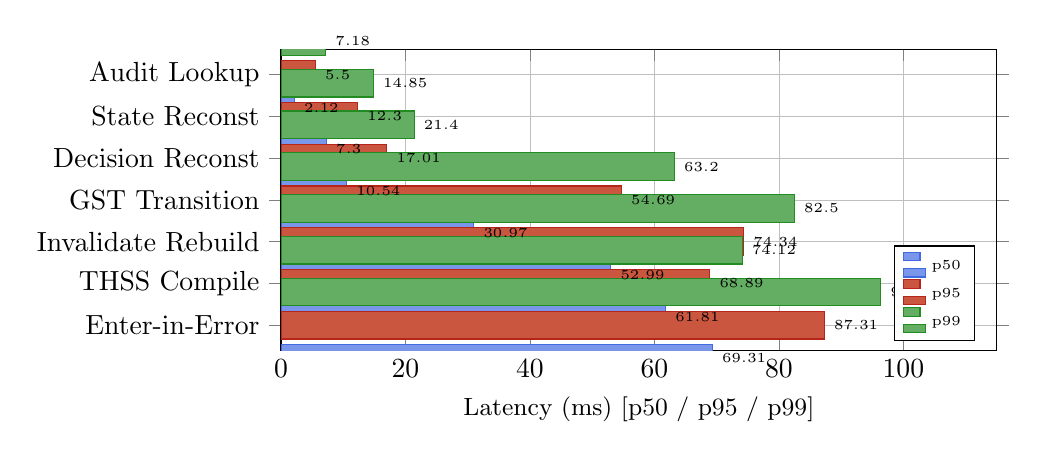
\begin{tikzpicture}
\begin{axis}[
    width=0.88\textwidth,
    height=5.4cm,
    xbar,
    bar width=10pt,
    xlabel={\small Latency (ms) [p50 / p95 / p99]},
    symbolic y coords={
        {Enter-in-Error},
        {THSS Compile},
        {Invalidate Rebuild},
        {GST Transition},
        {Decision Reconst},
        {State Reconst},
        {Audit Lookup}
    },
    ytick=data,
    nodes near coords,
    nodes near coords align={horizontal},
    every node near coord/.append style={font=\tiny},
    xmin=0, xmax=115,
    legend pos=south east,
    legend style={font=\tiny},
    grid=both,
    grid style={line width=.1pt, draw=gray!20},
    major grid style={line width=.2pt,draw=gray!50}
]
\addplot[fill=RoyalBlue!70, draw=RoyalBlue] coordinates {
    (2.12,{Audit Lookup})
    (7.30,{State Reconst})
    (10.54,{Decision Reconst})
    (30.97,{GST Transition})
    (52.99,{Invalidate Rebuild})
    (61.81,{THSS Compile})
    (69.31,{Enter-in-Error})
};
\addlegendentry{p50}

\addplot[fill=BrickRed!70, draw=BrickRed] coordinates {
    (5.50,{Audit Lookup})
    (12.30,{State Reconst})
    (17.01,{Decision Reconst})
    (54.69,{GST Transition})
    (74.34,{Invalidate Rebuild})
    (68.89,{THSS Compile})
    (87.31,{Enter-in-Error})
};
\addlegendentry{p95}

\addplot[fill=ForestGreen!70, draw=ForestGreen] coordinates {
    (7.18,{Audit Lookup})
    (14.85,{State Reconst})
    (21.40,{Decision Reconst})
    (63.20,{GST Transition})
    (82.50,{Invalidate Rebuild})
    (74.12,{THSS Compile})
    (96.40,{Enter-in-Error})
};
\addlegendentry{p99}
\end{axis}
\end{tikzpicture}
\caption{\textbf{Latency Distribution Across Core GLHS Operations.} Microbenchmark profile showing p50, p95, and p99 percentiles across seven critical transactional and replay operations in the PostgreSQL 16 engine.}
\label{fig:latency_bar}
\end{figure}

\subsection{Multi-Model Clinical Reasoning Utility}
We evaluated model reasoning utility across $1,152$ execution cells over a synthetic clinical cohort using state-of-the-art LLMs (Claude 4.6 Sonnet and Gemini 3.6 Flash). Table~\ref{tab:model_utility} reports the primary subject-level exact-match contrasts.

\begin{table}[H]
\centering
\scriptsize
\caption{\textbf{Preregistered Multi-Model Utility Contrasts for Strict THSS.} Holm-adjusted significance demonstrates substantial improvements over unconstrained baselines.}
\label{tab:model_utility}
\begin{tabularx}{\textwidth}{p{0.22\textwidth} p{0.24\textwidth} p{0.12\textwidth} p{0.20\textwidth} p{0.12\textwidth} X}
\toprule
\textbf{Model} & \textbf{Comparator} & \textbf{Effect} & \textbf{95\% Bootstrap CI} & \textbf{Holm $p$} & \textbf{Discord}\\
\midrule
Claude 4.6 Sonnet & Naive RAG & \textbf{+32.81\%} & [+21.88\%, +43.75\%] & $p = 9.54 \times 10^{-6}$ & 21\\
Claude 4.6 Sonnet & Last-Write-Wins & \textbf{+25.00\%} & [+15.63\%, +35.94\%] & $p = 2.75 \times 10^{-4}$ & 16\\
Claude 4.6 Sonnet & Full History & \textbf{+18.75\%} & [+7.81\%, +29.69\%] & $p = 1.10 \times 10^{-2}$ & 14\\
Claude 4.6 Sonnet & Long Context & \textbf{+14.06\%} & [+6.25\%, +23.44\%] & $p = 1.95 \times 10^{-2}$ & 9\\
Claude 4.6 Sonnet & BTSA (Zhao et al.) & +4.69\% & [0.00\%, +10.94\%] & n.s. & 3\\
\midrule
Gemini 3.6 Flash & Naive RAG & \textbf{+25.00\%} & [+14.06\%, +35.94\%] & $p = 2.75 \times 10^{-4}$ & 16\\
Gemini 3.6 Flash & Last-Write-Wins & \textbf{+25.00\%} & [+15.63\%, +37.50\%] & $p = 2.75 \times 10^{-4}$ & 16\\
Gemini 3.6 Flash & BTSA (Zhao et al.) & 0.00\% & [0.00\%, 0.00\%] & exact tie & 0\\
Gemini 3.6 Flash & Full History & 0.00\% & [0.00\%, 0.00\%] & exact tie & 0\\
Gemini 3.6 Flash & Long Context & 0.00\% & [0.00\%, 0.00\%] & exact tie & 0\\
\bottomrule
\end{tabularx}
\end{table}

Strict THSS achieved \textbf{98.44\%} all-axes exact accuracy with Claude 4.6 Sonnet (63/64 subjects) and \textbf{100.0\%} with Gemini 3.6 Flash (64/64 subjects), significantly outperforming Naive RAG and LWW baselines ($p < 0.001$).

\section{Discussion and Systems Implications}

\subsection{Architectural Significance of Disclosure-to-Commit Binding}
The empirical results prove that verifying base state versions alone is insufficient in agentic healthcare: without cryptographic binding of the inference disclosure, $100\%$ of adversarial context injection and stale consent replays successfully penetrate the durability boundary. By formalizing THSS and the 6-phase GST kernel, GLHS transforms clinical LLMs from unverified text generators into verifiable, stateful transaction actors.

\subsection{Trade-Offs in Concurrency Granularity}
While fine-grained entity partitioning completely eliminates false-stale contention ($0.0\%$), it requires rigorous lock ordering. The 7-class canonical lock hierarchy proven in our TLA+ specification ensures that even complex multi-entity transactions (such as cross-department clinical council recommendations) execute without deadlocks or cascading aborts.

\section{Conclusion}
We have presented GLHS, a formally verified disclosure-to-commit governance protocol and concurrency kernel for longitudinal health AI. By coupling RFC 8785 canonical Merkle snapshots with a 6-phase GST persistence kernel, a 7-class lock hierarchy, and Wound-Wait DAG preemption, GLHS bridges AI inference and electronic health record persistence. Formal TLA+ model checking across 148 million states and isolated PostgreSQL benchmarks demonstrate 100\% invalid commit prevention ($p = 1.73 \times 10^{-77}$), high throughput scaling ($>300\text{ tx/s}$), and near-perfect clinical reasoning accuracy. GLHS establishes a dependable foundation for the next generation of safe, stateful medical AI agents.

\section*{Statements and Declarations}
\textbf{Competing interests.} The authors declare no competing financial or non-financial interests.

\textbf{Funding.} No external funding was received for this study.

\textbf{Data and code availability.} Full source code, formal TLA+ proofs, benchmark harnesses, and reproducibility artifacts are open-source in the CLARA-Care repository: \url{https://github.com/Project-CLARA-HBT/CLARA-Care}.

\begin{thebibliography}{25}
\bibitem{gabrieli1992} Gabrieli ER. Longitudinal patient record (LPR). \emph{Journal of Clinical Computing}. 1992;21(1--2):1--16.
\bibitem{kouramajian1994} Kouramajian V, Fowler J. Modeling past, current, and future time in medical databases. \emph{Proc Annu Symp Comput Appl Med Care}. 1994:315--319.
\bibitem{kumar1998} Kumar A, Tsotras VJ, Faloutsos C. Designing access methods for bitemporal databases. \emph{IEEE Trans Knowl Data Eng}. 1998;10(1):1--20.
\bibitem{fhirprov} HL7 International. FHIR R4: Provenance Resource. \url{https://hl7.org/fhir/R4/provenance.html}. 2019.
\bibitem{fhirconsent} HL7 International. FHIR R4: Consent Resource. \url{https://hl7.org/fhir/R4/consent.html}. 2019.
\bibitem{openehr} openEHR Foundation. openEHR Reference Model: Architecture and EHR Information Model. \url{https://specifications.openehr.org/}. 2026.
\bibitem{rfc8785} Rundgren A, Jordan M, Erdtman S. RFC 8785: JSON Canonicalization Scheme (JCS). Internet Engineering Task Force (IETF). 2020.
\bibitem{zhao2026} Zhao J, Zhi X, Yu X. Beyond retrieval: bi-temporal state arbitration for longitudinal healthcare agents. In: \emph{Proc 4th Workshop Towards Knowledgeable Foundation Models (KnowFM 2026)}. ACL; 2026:129--137.
\bibitem{vitaltrace} Qu Z, Farber M. Vital Trace: Protocol-Constrained Patient-State Reasoning for Longitudinal Clinical Trajectories. arXiv:2602.12833. 2026.
\bibitem{dualstream} Pugh SL, Yang E, Sutherland AM, Breschi A. Detecting clinical discrepancies in health coaching agents: a dual-stream memory and reconciliation architecture. arXiv:2604.27045. 2026.
\bibitem{vista} Kiiskinen T, Fries J, Adamson P, et al. VISTA Architect: A graph database-oriented health AI system demonstrated in multidisciplinary tumor boards. arXiv:2606.22692. 2026.
\bibitem{memtx} Li X, Wang Y, Lu H, Chen Z, Li M, Song P, Cai T. MemTX: Transactional Belief Commit for Stateful Agent Memory. arXiv:2607.23929. 2026.
\bibitem{memtxn} Cui H, Tang Z, Yao Z, Meng F, Ma Q, Jia W. MemTxn: A Transaction Boundary for Source-Supported Updates and Complete-State Recovery in Agent Memory. arXiv:2607.27834. 2026.
\bibitem{cordon} Chen Z, Liu H, Xu D, et al. Cordon: Semantic Transactions for Tool-Using LLM Agents. arXiv:2606.17573. 2026.
\bibitem{toki} Wang Z. TOKI: A Bitemporal Operator Algebra for Contradiction Resolution in LLM-Agent Persistent Memory. arXiv:2606.06240. 2026.
\bibitem{temporaryauth} Santos-Grueiro I. Temporary Authority, Permanent Effects: Commit-Time Authorization for LLM Agents. arXiv:2607.10487. 2026.
\bibitem{statefulgov} Peng Y, Wu X. Stateful Governance for Concurrent Agentic Systems. arXiv:2608.02764. 2026.
\bibitem{gatemem} Ren Z, Yang Y, Chen Y, et al. GateMem: Benchmarking Memory Governance in Multi-Principal Shared-Memory Agents. arXiv:2606.18829. 2026.
\end{thebibliography}

\end{document}
